\documentclass{article}

\usepackage[utf8]{inputenc}

\usepackage[T1]{fontenc}

\usepackage{geometry}
\geometry{a4paper}

\usepackage[english]{babel}

\usepackage{setspace}
\doublespacing

\usepackage{amsfonts}

\usepackage{amsmath}

\usepackage{bm}

\usepackage{tikz}
\usetikzlibrary{trees}

\title{Signaling Game Ad Exchange}

\author{David Kasofsky}

\date{May 1, 2016}

\begin{document}

\maketitle

\newpage

\tableofcontents

\newpage

\section{Introduction}

TODO

\subsection{Motivation}

TODO

\newpage

\section{Ad Exchanges}

\subsection{Publishers, Consumers, and Advertisers}

In online advertising, publishers are those with ad space to sell. Publishers control websites which create and publish content, much of which is freely accessible, and wish to monetize the site traffic the content generates. TODO: this is a non sequitur, no mention of ad exchanges thus far etc. Without ad exchanges, publishers could only sell their ad space through deals negotiated directly with individual advertisers.

A publisher may represent a single site or multiple sites with different types of content. For our purposes, we will also consider search engines such as Google and Bing to be publishers although they are treated somewhat differently in practice. The challenge for publishers is to sell their ad space at the highest price || to maximize revenue via sale of ad space. In general, there are thousands if not millions of publishers registered with an ad exchange(FIND REFERENCE TO SUPPORT THIS)

Consumers visit publishers sites. As we know, hundreds of millions 

Advertisers purchase ad space in order to interact with consumers via advertisements. They are usually businesses or advertising agencies acting on behalf of businesses. Advertisers allocate a portion of their total marketing budget to be spent online. The challenge for advertisers is to find cost effective ad space on which to spend their online budget. 

TODO: reword

Common criteria to evaluate the potential of a publisher's ad space include the reputation of the publisher, consumer demographics that commonly visit the publisher's sites, and the alignment of the site's content with the advertiser's products. Once ad space has been purchased its performance may be evaluated using a process known as Attribution, which will be discussed later in great detail.

\subsection{The Funnel}

TODO: write this section ;)

\subsection{Role of the Ad Exchange}

An Ad Exchange is both an aggregator of publisher inventory and a marketplace for that inventory. This is good for publishers because listing their inventory on ad exchanges makes it easily available to a wide variety of advertisers. Publishers provide metadata about their listings, such as the type of content or the demographics which are likely to visit the publishers' sites. This in turn makes it easier for advertisers to find promising ad space.

TODO: mention varying quality of publisher-supplied metadata

In order to list their inventory with an exchange, a publisher signs up with and receives code from the exchange (e.g. some JavaScript) which allows ads to be dynamically inserted on the publisher's site(s). For example if the publisher's site layout includes a banner ad along the side of the page, the publisher will put the exchange's code in the spot a static banner ad would go.

Advertisers buy the listed ad space in auctions. Whenever a consumer visits a publisher's page which contains an exchange's code, the exchange is signaled that there is an opportunity to show an ad. Showing an ad to a consumer is called an "impression" and so we say an impression is available. The advertisers on the exchange then evaluate the impression and places bids according to their evaluation. The winning advertiser's ad is shown on the page. This whole process occurs in milliseconds so that the ad is loaded along with the rest of the content with no apparent delay to the consumer.

Because publishers provide metadata about their ad space, advertisers can include it in their evaluation. This highlights an important feature of ad exchanges: the ability to set bidding strategies according to impression metadata. As an impression auction must be resolved quickly, any logic to determine bid amounts is set ahead of time and is known as a bidding strategy.

The following are examples of an advertiser's potential bidding strategies:

\begin{itemize}
\item Bid \$0.50 for impressions on sites with many male visitors
\item Bid \$1 for impressions on sites with many male visitors between the ages of 20 and 40
\item Bid \$1 for impressions on Sports sites
\item Bid \$2 for impressions on Baseball sites but not between 1AM and 6AM
\end{itemize}

These illustrate how publisher metadata can influence advertisers' bidding strategies as well as publisher-independent factors such as time of day. Thus advertisers may have significantly differing evaluations of individual impressions. Such variation is the primary motivation for the use of auctions.

Let us consider why an advertiser would bid more for certain impressions. Plainly a higher bid implies a greater evaluation by the advertiser, i.e. greater anticipated ROI. There are ultimately two qualities of an impression which affect ROI: Conversion Rate and Conversion Revenue. Conversion Rate, known as CVR in the digital advertising world, is the probability of conversion given an ad interaction. Conversion Revenue is the amount of revenue a conversion generates. This could be an exact value, e.g. the purchase of a specific product, or modeled / approximated. Thus an impression with metadata $i$ could be evaluated with:

$ value_{i} = (1-\prod_{c \in C} 1-CVR_{c,i} ) (\sum_{c\in C} \frac{CVR_{c,i} \cdot revenue_{c}}{\sum_{c' \in C} CVR_{c',i}}) $
 
\noindent where $C$ is the advertiser's set of converting events, $revenue_{c}$ is the amount of revenue associated with conversion event $c$, and $CVR_{c,i}$ is the estimated conversion rate and revenue for conversion type $c$ for impression metadata $i$. The first term is the probability that a conversion occurs and the second term is the expected revenue.

The use of auctions highlights two major difference between buying on the exchange and buying directly form publishers. First, ads are usually bought from publishers using a constant rate, such as a cost per click (CPC) or a cost per thousand impressions (CPM). Second, some number of impressions are usually guaranteed. Thus an advertiser may pay a \$3 CPM for 1 million impressions per month, or exactly \$3,000 per month. This is a common type of directly negotiated deal. Since ad exchanges use auctions to sell impressions as they become available, there is no guaranteed number of available impressions and the price may vary from impression to impression. Therefore online advertising campaigns that spend heavily on ad exchanges usually require significantly more oversight and management than those of mostly direct deals.

\subsection{Third Party Data}

Third party data is data about consumers that has been collected and aggregated by third parties, i.e. neither publishers nor advertisers. In digital advertising the businesses that do so are known as Data Management Platforms (DMPs). A brief description is available at \cite{iab1}. Examples of such companies are Lotame and  BlueKai. Generally these companies gather data about consumers by partnering with various large e-commerce sites and monitoring activity on those sites. DMPs then make their consumer data available for purchase by advertisers who use it to tailor marketing strategies, e.g. by targeting consumers with specific features.

Whereas impression metadata only describes the site the ad will appear on, DMP data describes the consumer visiting the site. Consider the following bidding strategies:

\begin{itemize}
\item Bid \$1 on consumers on Sports sites
\item Bid \$1 on consumers with interest in Sports
\item Bid \$2 on consumers with interest in Sports on Sports sites
\end{itemize}

The first is a bidding strategies based on impression metadata only and the second based only on DMP data. The third combines both impression metadata and DMP data and shows more information about an impression can make it more valuable.

A major use of third party data is to supplement impression metadata in exchange auctions. Ad exchanges integrate with DMPs so that when an impression become available, the DMP's data can also be made available to advertisers. Advertisers pay a premium in order to use data from a DMP. In order to be competitive, bidding strategies which use DMP data must be more effective than those which do not.

Much third party data is collected and organized using cookies. First, a consumer is given a uniquely identifiable cookie the first time they visit a site which is monitored by a DMP. When that consumer visits certain pages or perform certain activities on the site or others monitored by the DMP, the DMP stores information related to the cookie id. For example, if a consumer visits a sporting goods site then the DMP may associate that consumer with the "sports" demographic.

Similar tracking is also used by ad servers. The first time a consumer receives an ad from a particular ad server, they are also given a uniquely identifiable cookie. This can be used to track which ads a consumer has been served. This will be seen to be critical in our discussion of Attribution.

Additionally, advertisers can use the ad server's tracking to associate data to cookie ids. Such information is known as first party data. A common tactic known as retargeting effectively flags consumers which have visited the advertiser's website and then pursues these consumers aggressively as they continue to browse the web. Many consumers have had creepy experiences where they encounter ads for products or brands they had recently viewed- this is retargeting.

It is important to note that cookie-based tracking has many issues as cookies cannot uniquely identify a single consumer across multiple devices or browsers. Other tracking methods are emerging to address this. For example, the Google Chrome browser encourages its users to sign in to the browser with their Google account. If a consumer does this, then Google achieves very reliable cross-device tracking of that consumer. A full discussion of such methods is out of the scope of this paper but further reading can be found in TODO need references here

\subsection{Attribution}

Before executing various advertising strategies, advertisers must decide on the events and activities they wish to cause by showing ads. When such an event occurs it is called a conversion and the associated consumer is said to have converted. The best example of conversions are purchases. Advertisers may record additional information such as the revenue generated by the conversion.

It is common for advertisers to define multiple types of conversions of potentially different values. Merely visiting the advertiser's homepage may be considered a type of conversion. Another common scheme is to have multiple conversion types which act as checkpoints within a longer process, e.g. for businesses that require customers to submit applications for approval.

Since causing specific types of conversions is an advertiser's goal, the advertiser must be able to associate conversions with ads in order to evaluate advertising strategies. In its simplest form, this is accomplished using the same tracking which associates ads to consumers. By assigning each consumer a unique identifier, usually a cookie id, the advertiser records which ads have been shown to that consumer as well as which, if any, conversions that consumer has performed.

However, it is not enough to simply associate ad interactions and conversions to consumers. Advertisers not only wish to know which ads a consumer has interacted with but also the effect each ad had. Consumers frequently interact with numerous ads and it is not clear which if any of the ads significantly impacted the consumer's decision to convert. If advertisers could accurately divide the credit for causing a conversion among the preceding ad interactions they could also do so with the associated revenue and thereby calculate the ROI for each ad.

The process of allocating credit for conversions to preceding ad interactions is called attribution. A particular mechanism for doing so is called an attribution model. The industry standard attribution model is Last Click. It attributes all credit for a conversion to the last-clicked ad or the last-viewed ad in lieu of a click. Plainly this does not capture the full detail of ad interaction but it has some motivating factors. It is very simple to understand as well as to implement. Variations include few parameters such as the maximum time between ad interaction and conversion for which the ad remains eligible. For instance, a click may become ineligible for credit after ten days but a view may become ineligible after five.

More sophisticated models are available to advertisers, usually from third parties. Example of such companies are Visual IQ and Adometry. These models are data-driven or algorithmic as compared to Last Click which is rule-based. Such models incorporate a statistical analysis to determine the chance of conversion given interactions with certain ads or combinations of ads and allocate credit for conversions accordingly. However many advertisers do not employ more sophisticated methods because of the additional cost, implementation difficulty, and lack of transparency when using a third party. TODO fix this description. weird and needs evidence to support

TODO: talk about how attribution fits into optimization / budget allocation

\subsection{Summary}

Publishers, Advertisers, DMPs, Attribution, and Ad Exchanges are the five pillars of digital marketing. Publishers represent supply while Advertisers represent demand. DMPs provide information about consumers while Attribution provides evaluations of advertising strategies. Ad exchanges are fluid, high-tech marketplaces which facilitate inclusion of third party data and allow timely responses to ad performance. Above all, ad exchanges make it easier for publishers and advertisers to meet their goals and to try new things. 

\newpage

\section{Signaling Games}

TODO: discuss crawford \& sobel

\subsection{Basic Model}

The crux of the signaling game is information asymmetry. One player has some information which is hidden from the other and wishes to convince the other to do something. Thus the informed player, called the Sender, must choose how to make his case while the second player, called the Receiver, must decide how to act based on the message from the Sender. As in typical game theory, both players wish to maximize their utility in this exchange. One can succinctly think of a signaling game definition requiring a sender, a receiver, some hidden information, the sender's possible messages, and the receiver's possible actions.

Such games are found to resemble interactions in nature, perhaps most famously described by Grafen \cite{grafen1} in his formalization of ideas from Zahavi \cite{zahavi1}. Here we see an example of signaling games used to describe mate selection. Consider a species in which the females choose which males to mate with and naturally want to select the best males. It is common for the male to signal his fitness by demonstrating a handicap, e.g. the cumbersome antlers of male deer. Since it is easier for healthier bucks to carry heavy antlers, antlers size generally indicates the buck's true fitness. In this the case the sender is the buck, the receiver is the doe, the hidden information is the fitness of the buck, the message is the size of antlers, and the action is to mate or not. 

Spence \cite{spence1} gives an example of how such games can model the hiring process. Here the sender is an applicant, the receiver is an employer, the hidden information is the competency of the applicant, the message is the credentials of the applicant, and the action is the wage offered to the applicant. Applicants want to be hired with the highest wage and employers want to pay applicants appropriately. Similarly to the antlers of deer, higher credentials are easier to earn for more competent applicants and so the employer may base his wages on the applicant's credentials.

A final example is Simple Poker. The sender has either a winning hand or a losing hand and can send one of two messages: Bet or Check. The sender's hand is hidden from the receiver can either Call or Fold. Here is the extensive form game:

\begin{figure}
\begin{center}
	\tikzstyle{level 1}=[level distance=1.5cm, sibling distance=6.75cm]
	\tikzstyle{level 2}=[level distance=1.5cm, sibling distance=3cm]
	\tikzstyle{level 3}=[level distance=1.5cm, sibling distance=1.5cm]
	\tikzstyle{level 4}=[level distance=1.5cm, sibling distance=2cm]
	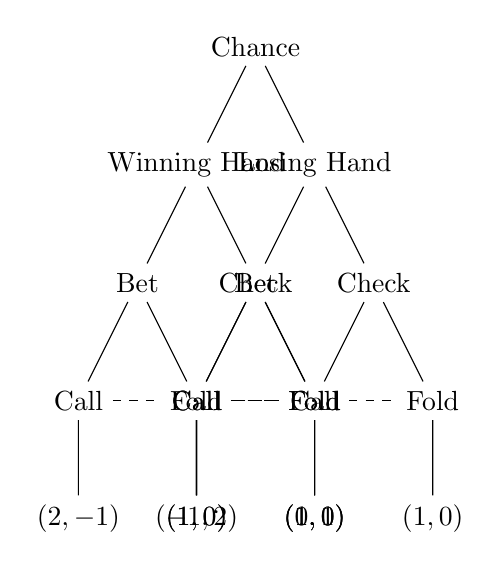
\begin{tikzpicture}
		\node{Chance}
			child{
				node(win){Winning Hand}
				child{
					node(wbet){Bet}
					child{
						node(wbcall){Call}
						child{
							node{$(2,-1)$}
							edge from parent
						}
						edge from parent
						node[left]{}
					}
					child{
						node(wbfold){Fold}
						child{
							node{$(1,0)$}
							edge from parent
						}
						edge from parent
						node[right]{}
					}
					edge from parent
					node[left]{}
				}
				child{
					node(wcheck){Check}
					child{
						node(wccall){Call}
						child{
							node{$(1,0)$}
							edge from parent
						}
						edge from parent
						node[left]{}
					}
					child{
						node(wcfold){Fold}
						child{
							node{$(1,0)$}
							edge from parent
						}
						edge from parent
						node[right]{}
					}
					edge from parent
					node[right]{}
				}
				edge from parent
				node[left]{}
			}
			child{
				node(lose){Losing Hand}
				child{
					node(lbet){Bet}
					child{
						node(lbcall){Call}
						child{
							node{$(-1,2)$}
							edge from parent
						}
						edge from parent
						node[left]{}
					}
					child{
						node(lbfold){Fold}
						child{
							node{$(1,0)$}
							edge from parent
						}
						edge from parent
						node[right]{}
					}
					edge from parent
					node[left]{}
				}
				child{
					node(lcheck){Check}
					child{
						node(lccall){Call}
						child{
							node{$(0,1)$}
							edge from parent
						}
						edge from parent
						node[left]{}
					}
					child{
						node(lcfold){Fold}
						child{
							node{$(1,0)$}
							edge from parent
						}
						edge from parent
						node[right]{}
					}
					edge from parent
					node[right]{}
				}
				edge from parent
				node[right]{}
			};
	\draw [dashed](wbcall)--(wbfold);
	\draw [dashed](wbfold)--(wccall);
	\draw [dashed](wccall)--(wcfold);
	\draw [dashed](wcfold)--(lbcall);
	\draw [dashed](lbcall)--(lbfold);
	\draw [dashed](lbfold)--(lccall);
	\draw [dashed](lccall)--(lcfold);
	\end{tikzpicture}
\end{center}
\end{figure}

To Bet signals a winning hand while to Check signals a losing one. The game is interesting because the sender may bluff by betting when he has a losing hand. 

With a few examples to build our intuition, we will shortly give a mathematical description of basic signaling games. We say basic here because we will extend this model in later games. First of all, a signaling game is a mathematical game like those studied in game theory. Game theory is generally interested in finding optimal strategies in multiplayer games. A game theoretical analysis almost always starts with assumptions about the goals, abilities, and rationality of the players, perhaps most importantly that the players will all play in such a way to maximize their score in the game. One can imagine player $i$'s score to be the output of some function $u_i$ and so $i$ will play so as to maximize $u_i$. This is a nice way to address arbitrary player preferences in complex or realistic games as such preferences are ultimately expressed by the value of $u_i$. 

These assumptions limit players' playable strategies, e.g. a player will not choose strategy A if it gives a lower score than strategy B. This brings us to the cornerstone of game theory: Nash equilibrium. A Nash equilibrium is a strategy assignment for each player such that each player's score is maximized given the strategies of the others. Thus a Nash Equilibrium is akin to a solution of a game since it gives each player a strategy which cannot be improved given the strategies of the other players.

It is important to note the difference between pure and mixed strategies. A pure strategy is deterministic while a mixed strategy is probabilistic. Recall the Simple Poker game from above. A pure strategy for the sender is to bet winning hands and check losing hands. The best response for the receiver is then to fold to all bets and call all checks. Note that this pair of strategies is not a Nash equilibrium because the sender's best response to the receiver's strategy is to bet losing hands as well, since the receiver will fold to all bets. 

A mixed strategy would be to always bet a winning hand and bet a losing hand half of the time. This time, however, we have a hiccup in choosing the receiver's best response strategy. Suppose the receiver knows that the sender is betting half of his losing hands. The receiver still does not know how often the sender has a winning hand and so we need another tool in order to find the receiver's best response.

This brings us to the concept of Bayesian games. Signaling games are Bayesian games and thus so is the Simple Poker game. A Bayesian game is a game in which some information is hidden from the players. Here we should mention that the information can be hidden symmetrically, unlike in the case of the signaling game. One way to represent the hidden information is to a imagine a set $\Omega$, elements of which represent possible configurations of game variables. In the Simple Poker game, for example, $\Omega = \{\text{Winning Hand}, \text{Losing Hand}\}$. When a Bayesian game is initialized, an element of $\Omega$ is chosen and each player is assigned some probability distribution $\pi_{i}(\cdot)$ over $\Omega$, i.e. a prior belief over the possible variable configurations.

Now we can address the receiver's best response in the Simple Poker game when the sender plays a mixed strategy. Recall that even if we knew how much the sender was bluffing, we could not choose a best response without also considering how often the sender had a winning hand. Let us now suppose that the receiver believes the sender has a winning hand half of the time, i.e. $\pi_R(\text{Losing Hand}) = 0.5$. Now it is straightforward to pick the best response strategy. Instead of folding to all bets as in the pure strategy response, the receiver should now call one third of the bets the sender makes. This is because if the sender is betting all his winning hands and half his losing ones, he will bet three quarters of all his hands and one third of those bets will be bluffs. Naturally the values from the above payoff matrix were relevant in this reasoning but were chosen for our ease at this point.

With these concepts in hand, we can concisely describe the basic signaling game. There are two players, $S$ and $R$. $S$ has some type $t \in T$ which is known to $S$ but unknown to $R$. $T$ is analogous to the set $\Omega$ from before. Each player also has a prior $ \pi_i(dcot)$ over $T$. One can imagine $\pi_{S}$ assigns probability 1 to $t$ and $\pi_{R}$ does not, e.g. $\pi_{R}$ could assign uniform probability to each $t \in T$. $S$ chooses a message $m$ from a set $M$ which is sent to $R$. Considering $m$ in light of $\pi_R$, $R$ chooses an action $a$ from a set $A$. Each player then receives a score according to functions $u_R$ and $u_S$ : $T \times M \times A \to \mathbb{R}$.

A strategy for S is then a function $\mu_{S}: T \times M \to [0,1]$ such that $\forall t: \sum_{m \in M} \mu_{S}(t, m) = 1$, i.e. assigns a probability to each message for all types. A strategy for R is a similarly $\mu_{R} : M \times A \to [0,1]$ such that $\forall m: \sum_{a \in A} \mu_{R}(m,a) = 1$.

\subsection{Equilibria}

Three types of Nash equilibria exist in signaling games:

\begin{enumerate}
\item Separating Equilibria, in which each type of sender send different signals. That is:

$\forall t, t' \in T, \exists M_{t} \subset M$ with $\mu_S(t,m) > 0 \Rightarrow m \in M_{t}$ and $t \ne t' \Rightarrow M_{t} \cap M_{t'} = \emptyset$.

\item Pooling Equilibria, in which all types send the same message. That is: $\exists  m \in M, \forall t \in T : \mu_S(t,m) = 1$.

\item Mixed Equilibria, which fall into neither of the previous two categories. Senders of differing types may send the same messages but may not as well. 
\end{enumerate}

Because signaling games are games of information asymmetry, we can interpret strategies and equilibria in terms of deception. The informed player, S, can deceive the uninformed player R. Consider the Simple Poker game once more: to sometimes bet with losing hands is a deceptive strategy that exploits the receiver's ignorance. 

 For instance, a separating equilibrium suits games in which the sender and receiver have a common interest and so the sender does not necessarily wish to be deceptive. Rather the sender wants to confer the maximum amount of information about the hidden type via the signal.

In a separating equilibrium, the receiver is able to deduce the sender's type from signal. Since the sender's utility function $u_{S}$ and possible types $T_S$ are common knowledge, the receiver can deduce which signal would be sent by each type. This makes the receiver's choice of action straightforward.

In a pooling equilibrium, the sender confers no information about the hidden type as all senders send the same signal. In this case the receiver's strategy is independent of the signal and depends only on $\pi_{ R}$. This is maximally deceptive but so obviously as to render the signal meaningless.

\subsection{Costly Signaling}

Costly signaling is an important feature of many signaling games. Suppose $G$ is a signaling game with $M$ a real interval and consider $u_{S}(t,s,a)$.

\subsection{Iterated Signaling Games}

\subsection{Recommenders and Verifiers}

\subsection{Signaling Games in Advertising}

\newpage

\section{Signaling Game Ad Exchange}

Thus far we have discussed the general landscape of digital advertising, some basics of game theory and signaling games, and how signaling games appear in advertising. Now we move to a complex game of our own design: the Signaling Game Ad Exchange. Imagine consumers browsing the web, visiting various web pages that suit their interests. Some of these pages will be listed on ad exchanges. When a consumer visits such a page, advertisers on the exchange bid on the available impression and the winning advertising's ad appears on the page. The consumer may then interact with the advertiser's ad, perhaps leading to a conversion. One consumer may visit many web pages so an advertiser frequently interacts with the same consumer multiple times. Over time, advertisers can use attribution to identify which ads are the most effective and which DMPs provide the best third party data. Our goal is to plausibly describe this process using signaling games. We focus first on the two most important pieces: impression auctions and consumer-ad interactions.

As such we will have two categories of players in our game: Consumers and Advertisers. Consumers wish to browse the net without interruption, e.g. from irrelevant advertisements. Consumers also want to purchase products which suit them. Advertisers want consumers to buy their products and encourage them to do so by showing ads. To capture all of this, we think of our Signal Game Ad Exchange broken into three phases: the Auction Phase, the Ad Phase, and the Conversion Phase. In the Auction Phase, we play a signaling game called the Auction Game. The sender is a consumer and the receivers are $n$ advertisers. The consumer sends impression metadata, which is bid on by the receiving advertisers in an auction. The winning advertiser and the consumer go on to the Ad Phase. We play a signaling game called the Ad Game, in which the winning advertiser is the sender and the consumer is the receiver. The advertiser's sends an ad to be shown to the consumer and the consumer decides how to interact with the ad. After both games have been played, the Conversion Phase occurs. In this phase the consumer randomly decides whether to convert, i.e. to buy an advertised product. This completes an iteration of the Signaling Game Ad Exchange. Utility functions are calculated in each phase of the game and a player's ultimate utility is the sum of the utilities calculated in each phase. TODO: insert figures

As both consumers and advertisers may play the role of sender, players from each category have associated types. The type space $T$ is the set of unit vectors in $\mathbb{R}^N$. The type of player $i$ is then some $t_i \in T$. Player type vectors should be interpreted as a list of product affinities. We imagine that there are different products or features of products; thus a consumer type vector describes the products the consumer would like to buy and an advertiser type vector describes the products the advertiser promotes.  As in the classic signaling game, each player $i$ knows only his own type $t_i$. The players' beliefs about unknown information in the game is represented by a Bayesian prior $\pi_i$ over $\Omega$, where $\Omega$ is the set of possible game variable configurations. 

So far we have introduced two hyperparameters of the game. $N$ is the number of products, which determines the dimension of the player types and, as we will see, their messages. $n$ is the number of advertisers which participate in the impression auctions. We will continue to refer to these hyperparameters throughout the following discussion of the Auction Phase and the Ad Phase. 

\subsection{Auction Phase}

In the first phase, the Auction Phase, we simply play a signaling game modeling an impression auction on an ad exchange. We call this the Auction Game. Here the sender is a consumer and the receivers are the $n$ advertisers who will bid on the impression. Consumers' messages represent impression metadata. Consumers choose the sort of impression metadata which is relayed to advertisers on the exchange by visiting certain types of sites. While the ad exchange technically delivers the impression metadata to advertisers, it is the consumer who determines its content. The consumer message space $M$ is again the set of unit vectors in $mathbb{R}^N$. The components of a consumer message vector $m \in M$ similarly correspond to product affinities, in this case for the web page the consumer is visiting. One can imagine that different types of web pages, various e-commerce pages in particular, could be more or less associated with certain types of products.

The advertisers on the exchange receive the impression metadata and must decide how much to bid for the available impression. The bid amount $\beta$ is the advertiser's action. The action space $A$ is the set of non-negative real numbers, $\mathbb{R}^{\ge 0}$. Each of the advertiser's bids are entered in a Vickrey auction \cite{vickrey_auctions} and the winner goes on to play the Ad Game. A Vickrey auction is a sealed price auction in which the winner pays the amount of the second-highest bid. A sealed-price auction is one in which bids are given without knowing the bids of other participants. This type of auction has been shown to encourage truthful bids (in particular circumstances), i.e. bids that reflect the bidder's actual evaluation of the item at auction. A generalized version, though with significantly different properties, is commonly used in the auction of search keywords \cite{edelman_gsp}. We choose this type of auction because of its influence on the development of auctions in digital advertising, e.g. the aforementioned search keyword auctions.

With the sender's messages and receivers' actions in hand, we may turn to the players' utility functions. The consumer's utility function $u_{auction_S}$ is the dot product of consumer's type and the impression metadata, i.e. $t_S \cdot m$. The intuition here is that the consumer's primary goal is to visit websites which suit their interests. Since consumer type and impression metadata are both unit vectors, the dot product is equal to the cosine of the angle between the vectors. Thus we interpret larger cosine, i.e. smaller angle between vectors, as a better match between taste (consumer's type) and content (impression metadata). A better match between consumer type, i.e. taste, and impression metadata, i.e. content, is better for the consumer. Now, at this point one may wonder how the advertisers' actions affect the consumer since they do not affect the utility function. The answer is they will affect the consumer's utility in the second game, the Ad Game.

The advertisers' utility function $u_{auction_R}$ is merely the auction result: the winning advertiser receives negative utility equal to the second highest bid and the others receive zero utility. The negative utility corresponds to the amount the winning advertiser must pay in order to show an ad. Once again, the consumer's message and type are absent from the utility function at this stage but will affect the advertiser's payoff in the ad game.

Let $U^N$ be the set of unit vectors in $\mathbb{R}^N$. We may summarize the game definition thus far as follows:

\begin{itemize}
	\item The sender $S$ is a consumer with type $t_S \in T_S = U^N$.
	\item The receiver $R$ is a set of advertisers, $R = \{r_1, r_2, ... r_{n-1}, r_n \}$, each with type $t_{R_i} \in T_R = U^N$.
	\item The message space $M$ = $U^N$ is the set of possible impression metadata sent by $S$.
	\item The action space $A = \mathbb{R}^{\ge 0}$ is the set of possible bids by members of $R$.
	\item The sender's utility function $u_{auction_S}(t_S, m) = t_S \cdot m$ where $m \in M$.
	\item The receivers' utility function $u_{auction_R}(a_1, a_2, ... a_{n-1}, a_n)$ is the Vickrey auction result.
\end{itemize}

\subsection{Ad Phase}

In the second phase, the Ad Phase, we play a signaling game modeling a consumer-ad interaction. We call this the Ad Game. The roles are reversed from the the Auction Game: the sender is an advertiser and the receiver is a consumer. The advertiser's message represents an ad, e.g. a banner ad. Ads are represented by $N$-dimensional unit vectors, the components of which once again correspond to product affinities. However: an advertiser may not simply send whatever message they chose. Instead, messages for advertiser $j$ are constrained to a set $M_j$ of size $\alpha$, $\alpha$ another hyperparameter of the game. The intuition is that an advertiser does not have myriad ads at his disposal. Instead advertisers must work with a small number, e.g. $\sim 10$, available ads and aim to deliver the most suitable ad he can. Additionally, advertisers do not know $\emph{a priori}$ which ads are best suited to particular situations. As ad messages are represented by vectors of product affinities, these vectors are akin to the types of the ads. So, much like advertisers do not know the types of consumers, advertisers do not know the types of their ads. Advertiser's beliefs about the types of their ads are reflected by the prior $\pi_i(\cdot)$.

The consumer receives the ad and must decide how to interact with it. The amount of interaction is represented by a number in $[0,1]$, with a higher value representing more interaction with the ad. Today's ads are quite sophisticated and interactive. As such, an ad may relay all kinds of consumer interaction data back to the advertiser. For example, a video ad will track how much of the video the consumer watches as well as whether they pause, restart, mute, full-screen, etc. Other ads may have interactive features like buttons, carousels of products, and mini-games and track how these features are used by a consumer. Thus there is a spectrum of possible ad interactions and the depth of interaction in particular instances is visible to the advertiser.

The advertiser simply receives 0 utility for this game, i.e. $u_{ad_S}(\cdot) = 0$. Because ad interaction does not generate revenue, the advertiser does not receive any explicit value from it. Instead the advertiser is hoping it pays off later in the form of a revenue-generating conversion which may occur in the Conversion Phase. The consumer utility function $u_{ad_R} = -a$, where $a$ is the amount of ad interaction. This is because ad interaction is a detraction from the consumer's regular browsing. However: consumers do wish to purchase suitable products and may only learn about them through advertising. Thus there is an incentive to interact with advertising as it may lead to a purchase.

Let us offer a short summary of the Ad Game:

\begin{itemize}
	\item The sender is an advertiser $\alpha_j$ with type $t_j$.
	\item The receiver is a consumer $\gamma_i$ with type $t_i$.
	\item The message space $M_j \subset U^N$ is the set of ads available to $\alpha_j$.
	\item The action space $A = [0,1]$ represents the possible amounts of consumer-ad interaction.
	\item The sender's utility function $u_{ad_S}(\cdot) = 0$.
	\item The receivers utility function $u_{ad_R}(a) = -a$, where $a \in A$.
\end{itemize}

\subsection{Conversion Phase}

At the conclusion of the Ad Phase, two random events occur. The first is consumer state transition. Consumers not only have a type but a dynamic state. A consumer's state, motivated by the marketing funnel, represents their interest in a certain product and hence their chance to convert. A consumer has a state with respect to each advertiser. The possible consumer states are:

\begin{enumerate}
	\item Ignorance: the consumer is ignorant of the advertiser and will convert with probability $p_Ignorance = 0$.
	\item Awareness: the consumer is aware of the advertiser and will convert with probability $p_Awareness << 0.01$.
	\item Interest: the consumer is interested in the advertiser and will convert with probability $p_Interest \sim 0.01$.
%	\item Rejection: the consumer has rejected the product and will convert with probability $p_Rejection = 0$s
TODO: rejection / adblock state to go in future directions
\end{enumerate}

A consumer's initial state with respect to an advertiser is determined by the choice of $\omega \in \Omega$. The states are ordered Ignorance, Awareness, Interest and consumers may only transition to the next state or remain in their current state. A consumer transitions to the next state with probability $max(0, a (t_i \cdot m_j))$, where $a$ is the amount of advertising interaction in the Ad Game, $t_i$ is the consumer's type, and $m_j$ is the ad sent by advertiser $j$ in the Ad Game. Recall $a \in [0,1]$ and $t_i \cdot m_j \in [-1,1]$ so that $max(0, a (t_i \cdot m_j)) \in [0,1]$. This means that consumers will have a higher chance to progress in the funnel the more they interact with an ad or the better an ad suits them. Ads that are unsuitable, i.e. have negative dot product, have no chance at affecting a consumer's state. See figure for state diagram.

TODO: insert figure

TODO: state with respect to product or advertiser? downside of with respect to advertiser is that advertiser's don't directly compete, e.g. one advertiser's ads may cause a consumer to transition to lower states in the funnel before receiving ads from a similar advertiser. downside of per product is that with unit vectors, it's not clear that a product per component interpretation is accurate. maybe that's better though.

Finally the consumer converts for each advertiser with probability according to their state with respect to that advertiser. Converting puts the consumer into a final pseudo-state ("converted") in which the consumer may not convert again for the same advertiser. The consumer and advertiser each receive 0 utility when there is no conversion. When there is a conversion for advertiser $j$ receives utility $v_j$, where $v_j$ is the value of the advertiser's product. The converting consumer $i$ receives utility $(t_i \cdot t_j) v_i$. That is, the consumer receives a fraction of the value of the product proportional to the alignment of $i$ and $j$'s type vectors.



\subsection{Third Party Data as Recommendation}

\subsection{Attribution as Verification}

\subsection{Consumers}

First, let us give a formal definition of a Consumer player. We will then address each attribute in detail.

A Consumer $C_i$ is a tuple $\langle t_i, f_i \rangle$ where:

\begin{itemize}
	\item $t_i \in U^N = \{\bm{x} | \bm{x} \in \mathbb{R}^N \wedge ||x|| = 1\}$ is the consumer's type
	\item $f_i \in F = \{ignorance, awareness, consideration, intention\}^N$ is the consumer's initial state in the funnel for each existing product type. 
\end{itemize}

Consumers in our game represent web-browsing consumers in real life. Each consumer player has a type $t_i$ which describes affinities for various types of products. These product affinities are represented by a $N$-dimensional unit vector, $N$ being a hyperparameter of the game. Each component of the consumer type vector corresponds to an affinity for a type of product. For example, a consumer with type vector $\rbrack 1, 0 \lbrack$ has an affinity for the first product but not for the second. The distribution used to generate a consumer's type vector is also a hyperparameter of the game.

Consumers' messages represent impression metadata, as a consumer is the sender in the Auction Game. In essence, consumers choose the sort of impression metadata which is relayed to advertisers on the exchange by visiting certain types of sites. While the ad exchange technically delivers the impression metadata to advertisers, it is the consumer who determines its content. A consumer message, i.e. impression metadata, is also presented as a $N$-dimensional unit vector. The components of the impression metadata vector once again correspond to product affinities but for the web page the consumer is visiting. One can imagine that different types of web pages, various e-commerce pages in particular, could be more or less associated with certain types of products. 

Consumer actions correspond to advertising interactions. Recall the Consumer plays the role of receiver in the Ad Game. The set of possible consumer actions $A_{Consumer}$ is $\{view, click\}$. An $impression$ interaction means that the ad was displayed on the page but the consumer did not click on it where a $click$ interaction signifies that the consumer did click on the ad and was therefore linked to the advertiser's website. We also associate these actions with the probability of a consumer state transition. As described in the first section, advertisers believe in the marketing funnel and that consumers can be more or less receptive to advertisements depending on their position in funnel. So each consumer not only has a hidden type but also a hidden state $f_i$ which corresponds to their position in the funnel for each product type. We use a four-stage funnel $F$ with states $\{ignorance, awareness, consideration, converted\}$. 

The intuition is that consumers with affinities for certain types of products are more likely to visit sites related to those products.

TODO: fix up this state stuff.
TODO: mere-exposure effect https://en.wikipedia.org/wiki/Mere-exposure\_effect
After each iteration of Auction Game and Ad Game, a consumer may convert, i.e. buy an advertiser's product.

TODO: conversion should occur randomly and separately from ad interactions

\subsection{Advertisers}

Again, we will begin with a formal description of an Advertiser player:

An advertiser $V_j$ is tuple $\langle t_j, \alpha_j \rangle$ where:

\begin{enumerate}
	\item $t_j \in [-1,1]^N$ is the advertiser's type
	\item $D_j$ is the set of ads available to the advertiser
\end{enumerate}

\newpage

\section{Ad Exchange Simulation}

\subsection{Agent-based Model}

\subsection{Simulation Details}

\subsection{Implementation}

Such messages are generated by rotating the consumer's type vector a random amount. Both the amount and direction of the rotation are randomly chosen at the time a message is generated. The rotation is achieved in the following way. Suppose we have a consumer with type $t_i = \frac{\bm{x}}{||\bm{x}||}$ where $\bm{x} \sim D$, e.g. the components of vector $\bm{x}$ are drawn i.i.d. from some distribution $D$. A message vector $m$ is then by $\frac{t_i + \bm{y}}{||t_i + \bm{y}||}$ with $\bm{y} \sim D$. This means that the expected value of the angle between a consumer's type and one of that consumer's messages is zero. The intuition is that consumers are likely to visit sites which suit their interests. Since consumer messages represent impression metadata and impression metadata represents the type of web site the consumer is visiting, it is likely that the impression metadata represents the consumer's type. However, there is no limitation on $D$ and so could may be plenty of variance in a consumer's messages.

\newpage

\section{Simulation Results}

\subsection{Summary}

\subsection{Naive Attribution}

\subsection{Improved Attribution}

\section{References}

\bibliography{tesis}
\bibliographystyle{plain}

\end{document}

